

\documentclass{article}
\usepackage[utf8]{inputenc}
\usepackage{authblk}
\usepackage{setspace}
\usepackage{natbib}
\usepackage{hyperref}
%\usepackage{cite}
\usepackage[margin=1in]{geometry}
\usepackage{array}
\usepackage{graphicx}
\usepackage{caption}
\graphicspath{ {./figures/} }
\usepackage{subcaption}
\usepackage{amsmath}
\usepackage{lineno}
\usepackage{soul}
\usepackage{xcolor}
\sethlcolor{yellow}
\linenumbers

%%%%%%%%%%%%%%%%%
\title{Thesis Proposal} %emwJan2 -- you should start thinking of a title
\date{\today}
\author{Christophe Rouleau-Desrochers}

\begin{document}
%%%%%%%%%%%%%%%%%%%%%%%%%%%%%%

\maketitle

 %emwJan2 -- my comments are noted with this! My overview comments are at the end. I did not spell check etc. my comments so if something does not make sense, let me know!

%<><><><><><><><><><><><><><><><><><><><><><><><><><><><><><><><><><><><><><><><>
% INTRODUCTION %
%<><><><><><><><><><><><><><><><><><><><><><><><><><><><><><><><><><><><><><><><>
\section{Introduction}
% <><><><><><><><><><><><><><><><><><><><><><><><><><><><><><>
% SECTION 1.1. %
% <><><><><><><><><><><><><><><><><><><><><><><><><><><><><><>
\subsection{Climate change impacts on tree phenology}
Research from the past decades has shown convincing evidence that human activity is increasingly affecting many worldwide environmental processes \citep{ceballos_biological_2017,intergovernmental_panel_on_climate_change_ipcc_climate_2023,laurance_have_2007,parmesan_globally_2003}. 
This can be through land use change and loss, pollution, invasive species, resource overexploitation and climate change \citep{driscoll_biodiversity-crisis_2018,parmesan_poleward_1999,wu_key_2013}. 
 %emwJan2 -- see below for easy way to make PV into AV (you still have a lot of PV so keep working on reducing it) 
Though some immediate actions can mitigate these impacts (e.g. \citep{campbell_producing_2014}), reversing 150 years of human-induced greenhouse gas emissions is harder. These emissions have affected Earth's climate and are projected to keep changing it for many centuries \citep{intergovernmental_panel_on_climate_change_ipcc_climate_2023}. Yet, the extent of the consequences that a warming climate will have on biological processes is still debated \citep{huey_predicting_2012}, in part because it requires accurate predictions of current and future trends in some of the most reported and direct biological impacts of climate change, as I review below. And also because it requires understanding the complex additional effects of these impacts, which I propose to study for my thesis. \\
% emwJan2 -- the below sentence doesn't really fit for me with the flow of the paragraph -- I tried to change it (above) so it flows better into next section, but you should work on it a little more and make sure it says what you want.
% While there is a scientific consensus that observed climate change is human-caused \citep{intergovernmental_panel_on_climate_change_detection_2014,lynas_greater_2021,oreskes_scientific_2004}, the magnitude and the extent of the consequences that a warming climate will have on biological processes are still debatable \citep{huey_predicting_2012}.  \\

% <><><><><><><><><><><><><><><><><><><><><><><><><><><><><><>

% <><><><><><><><><><><><><><><><><><><><><><><><><><><><><><>
\textbf{Trends and drivers of spring and autumn phenological events} \\ 
 %emwJan2 -- I think the flow is good enough now, so please remove the info on the outline ... that is, all the '\textit{1.1.1.1. Changes in phenology:}' etc. and start working on the sub-headers you will actually keep 
The most frequently observed biological impact of climate change over the past decades is major changes in spring and autumn phenology---the timing of recurring life history events                                                                                                                                                                                                                                                                                                                                                                                                                                     \citep{parmesan_globally_2003,cleland_shifting_2007,lieth_phenology_1974,woolway_phenological_2021,menzel_european_2006}. Together, shifts in spring and autumn phenology modify when the growing season starts and when it ends. Understanding the consequences of changing growing season length on ecosystems requires understanding how much, and why it has changed \citep{duputie_phenological_2015}. \\ 

\textit{Drivers of spring phenology:} Spring phenological events (e.g. budburst and leafout) have been advancing from 0.5 \citep{wolfe_climate_2005} to 4.2 days/decade \citep{chmielewski_response_2001,fu_recent_2014} and are mainly driven by temperature \citep{chuine_why_2010,cleland_shifting_2007,penuelas_responses_2001}. In the winter, when trees are still in dormancy, they accumulate cold temperatures (chilling) for which a certain amount is required to be ready to accumulate heat (forcing) \citep{vitasse_interaction_2014}. Then, in the spring, a certain amount of forcing triggers budburst \citep{fu_declining_2015}. Heat requirements are met sooner in warm springs, thus explaining the advancement of spring events and earlier onset of growing seasons over the last decades \citep{fu_declining_2015,fu_sensitivity_2013, laube_chilling_2014}. \\ 

\textit{Drivers of autumn phenology}: In contrast, autumn phenology (e.g. budset and leaf senescence) has delayed with climate change---though shifts in the autumn have been much smaller than those in the spring \citep{gallinat_autumn_2015,jeong_macroscale_2014}---and its drivers are also far less understood. These differences may be caused in part by the lesser attention payed to autumn phenology \citep{piao_plant_2019} and because the data is often noisier \citep{wu_canopy_2024}. However, some of these differences are likely due to different drivers of autumn phenology, as these phenophases appear to be driven by shortening photoperiod and colder temperatures \citep{cooke_dynamic_2012,flynn_temperature_2018,korner_phenology_2010,delpierre_temperate_2016}.  %emwJan2 -- you need a better connection OR transition between the drivers you mention here above and the ones below. So you either need to say something like -- 'Given that colder temperatures can lead to senescence, warmer autumns may delay leaf senescence, possibly by extending the activity of photosynthetic enzymes which causes decreases the degradation rate of chlorophyll. Additionally, drought .... ' OR you need spell out how these drivers work with CC and then say, additionally .... 
Given that colder temperatures can lead to senescence, warmer autumns may delay leaf senescence, possibly by extending the activity of photosynthetic enzymes which causes decreases the degradation rate of chlorophyll \citep{yan_divergent_2021}. Additionally, summer droughts could pause the activity schedule of trees and delay senescence to increase carbon assimilation \citep{dox_severe_2022}. Finally, there could be an antagonistic effect of warming and brightening---caused by reductions in atmospheric pollution and cloud cover \citep{sanchezlorenzo_reassessment_2015}---on leaf senescence \citep{wu_atmospheric_2021}. Brightening accelerates the leaf senescence processes and reduces the temperature sensitivity during that period, counteracting the expected warming-induced delays in leaf senescence \citep{wu_atmospheric_2021}. 
%emwJan2 -- Is there only ONE paper on this brightening idea? If so, I might skip it as you have a lot to explain already here ... if not, you should add a couple more citations.
% Vitasse 2021 showed something similar but for understory trees. but else, doesn't seem to be well supported. 
% <><><><><><><><><><><><><><><><><><><><><><><><><><><><><><>

% <><><><><><><><><><><><><><><><><><><><><><><><><><><><><><>
\textbf{1.1.2. How these shifts translate into effects on trees/forests is not clear - Pros and cons of early/late start/end of season} \\  %emwJan2 -- need a better subheader title 
 %emwJan2 -- below paragraph needs to mention your focus (and the literature that you cite) on trees/forests
Shifts in spring and autumn phenology in trees support a long-lasting and intuitive assumption that earlier spring and delayed autumn events lead to longer seasons---and thus increased growth \citep{keenan_net_2014, stridbeck_partly_2022}. However, research from the past three years has cast doubt on this hypothesis \citep{dow_warm_2022,green_limits_2022,silvestro_longer_2023}. For instance, \citep{dow_warm_2022} showed that despite an earlier growth onset, longer seasons did not increase the growth rate nor overall annual increment in trees. This could substantially affect forest carbon-cycle model projections on and thus feedbacks to future climate \citep{richardson_climate_2013,swidrak_comparing_2013}. Starting to grow earlier and stopping later both have different consequences (Figure 1).

% check that the sentence below doesn't repeat at the aims of my thesis
 %emwJan2 --  nice topic sentence! I also appreciate the more nuanced review of the source/sink debate
Understanding these findings requires answering why trees do not grow more despite longer growing seasons. While carbon allocation to above-ground biomass is one of the largest carbon sinks, how this carbon is allocated into wood is poorly understood. Indeed, the assumption of a linear relationship between wood growth and carbon assimilation is not well supported mechanistically and represents an important limitation of vegetation models \citep{cabon_cross-biome_2022}. Net primary production represents the difference between photosynthesis and plant respiration, but this commonly used metric completely omits the representation of growth processes. This is perhaps because of a long-lasting paradigm of source-limited photosynthesis \citep{friend_need_2019,parent_modelling_2010}. Whether a tree's growth is source (photosynthetic activity determines sink activity) or sink (growth, respiration, and other metabolic processes determines the carbon source) controlled depends upon a closely coordinated sequence of dynamic responses and is still an area of active debate. However, \cite{gessler_beyond_2024} recently suggested that neither source or sink control systematically dominate. This complex dynamic enforces the importance of understanding the temperature sensitivity relationship between growth activity and photosynthesis. Growing evidence suggests that cambial activity may be more sensitive than photosynthesis to a range of environmental conditions, such as water and nutrient availability, and temperature \citep{cabon_cross-biome_2022,cabon_water_2020,muller_water_2011,peters_turgor_2021}. Thus, this demonstrates that carbon projection models that solely rely on vegetation alone may mislead carbon sequestration dynamics of our forests. \\

% <><><><><><><><><><><><><><><><><><><><><><><><><><><><><><>
\textbf{1.1.3. Growing season shifts and consequences on forest ecosystems and services} \\ 
Spring and fall phenological events are shifting with debatable consequences on tree growth. The sensitivity of cambial activity to water, temperature and nutrients has the potential to have far-reaching consequences given the hard-to-predict nature of future climate change, where any of these variables could vary from low to high amplitude \citep{almagro_longterm_2025,cabon_cross-biome_2022}. This expected asymmetry of future environmental changes makes understanding the internal physiological constraints (via genetic and developmental control), and external limits (via extreme temperatures or moisture deficit) to growth critical, which I aim to investigate with experiments and observations.  %emwJan2 -- I think you probably should sneak in the point somewhere that you will use experiments and observations,  but i I don't think the below adds much so I cut it. 
 % ... and empirical data coming from experiments, but also from ground observations are paramount to predict the changes of forest carbon offset from human GHG emissions \citep{wolkovich_why_2025}.  


% <><><><><><><><><><><><><><><><><><><><><><><><><><><><><><>
% SECTION 1.2 %
% <><><><><><><><><><><><><><><><><><><><><><><><><><><><><><>
\subsection{Experiments and observations to understand the future of growth and season length relationship} %emwJan2 -- need a header more specific to your thesis

\textbf{1.2.1. Past phenological trends can help (or not) predict future phenological changes} \\ 
We cannot directly use observed phenological trends in the last decades to extrapolate future phenological changes because: (1) the mechanisms guiding them are not clear, and (2) phenological responses of trees to warming are very likely to be non-linear \citep{ettinger_winter_2020,fu_sensitivity_2013}. Indeed, accurate predictions require an in-depth, accurate mechanistic understanding of phenophases and their sensitivities to environmental drivers, especially to temperature and photoperiod \citep{fu_sensitivity_2013}. Therefore, the very foundation of the assumption that longer seasons increase growth may shift with future climate change. The well-observed advance in spring phenology may decelerate, and delayed fall phenology may shift towards earlier leaf senescence (through summer drought-induced growth cessation). \\

\textbf{1.2.2. The assumption that longer seasons lead to increased growth is called into question} \\ 
%emwJan2 -- you did a nice job removing a lot of repetitive stuff, except for the below which is SO similar to just two paragraphs before. You may consider opening with just a sentence like:  Recent work emphasizing the need to understand the drivers regulating growth across biomes has highlighted strong species-level variation that may be critical to accurate projections ... (or something like that). 
% Recent work shows an absence of increased growth despite apparent better environmental conditions, thus casting doubt on a simple and intuitive positive relationship between growing season length and growth. This paradox further emphasizes the need to better understand the drivers regulating growth across biomes, but also how these drivers vary across the species within these biomes. 
Recent work emphasizing the need to understand the drivers regulating growth across biomes has highlighted strong species-level variation that may be critical to accurate projections. 

Phenology varies greatly across species (e.g. closely related species tend to budburst at similar times under similar conditions) \citep{wolkovich_progress_2014}, but so does the relationship between growth and season length, which may explain the wide variation of this relationship within communities \citep{buckley_functional_2012}. This highlights another weakness of current carbon sequestration models that pool species together, likely overpassing important nuances in the growth responses that could be explained by species differences. Excluding species differences in models may mislead future carbon dynamic models \citep{green_limits_2022,cabon_cross-biome_2022,wolkovich_why_2025}. Different strategies can help understanding how different species respond to warming and thus improve carbon sequestration projections. \\

\textit{1.2.2.1. Experiments:} First, experiments are extremely useful in teasing apart co-occurring realities in natural environments. For example, warm springs, and severe droughts later in the summer often happen together within a single year making it difficult to tease these effects apart from observational data. Manipulative experiments, in contrast, have the capacity to separate the relative effect of each phenomenon\citep{morin_changes_2010,primack_observations_2015}, but also have major limitations, especially when working on trees. Logistical constraints of working with adult trees, mean that experiments are most often performed on juvenile trees. While saplings are critical for their role in forest regeneration projections, their responses often do not directly translate to mature trees, which hold the overwhelming carbon biomass proportion of forests \citep{augspurger_differences_2003,silvestro_longer_2023,vitasse_ontogenic_2013}. However, even if young trees are often more plastic than adult forms, their responses can still provide valuable insights in differences across species and populations \citep{wolkovich_why_2025}. \\

\textit{1.2.2.2. Ground based observations:} 
%emwJan2 -- some small flow problems below -- you have a good over-arching topic sentence, but you need to walk the reader through things more... I don't think you ever said that leaf phenology is accessible or what that means so you need to spell some of this out. You need to say that cambial phenology is a direct measure of wood growth, but super hard to get. in contrast, lead phenology ... --> Work on this and the general flow of this paragraph for next version. 
Second, leaf phenology  can provide valuable and accessible insights into the growth temporality of trees that are not suitable for experimental trials. Cambial phenology, which is a direct measure of wood growth, is very hard data to gather and requires expensive equipment (REF). In contrast, recording the timing of budburst or leaf colouring through ground-based observations are still low-cost methods that provide direct evidence of changing phenophases \citep{piao_plant_2019}. Cambial and leaf phenology are often closely synchronized, therefore, the more accessible leaf phenology data can act as a reliable proxy for the onset and end of tree growth. In other words, knowing when leaves elongate and colour can guide as to when trees start and stop growing, which is a fundamental metrics to determine the growing season length. Additionally, unlike other methods, ground observations have the advantage of providing accurate measurements of phenological events for specific sites and species. Recently, the widespread use of smartphones has considerably simplified the phenological monitoring by citizen scientists which has the potential to vastly increase the monitored areas and the range of studied species. \citep{dickinson_current_2012,hufkens_monitoring_2019,piao_plant_2019}. While there are drawbacks to observations by citizen science programs (e.g. non-standard protocols, highly uneven spatiotemporal distribution of these observations), they have a huge potential to diversify the phenology data. \\
% check back these two last sentences on citizen science programs

\textbf{1.2.3. Goals of my thesis}  \\ 
%emwJan2 -- I think you can add a REALLY nice transition sentence to the start of this paragraph below. I would use this as a chance to say that you aim to understand 'how different tree species, at different lifespan stages, vary in their growth responses to different season length' by working across different methods. .... then explain and introduce the names of your projects from one scale to another (I might start with fuelinex which is saplings to common garden to arb, but up you -- just pick an order and stick with it) ... then end on your nice transition sentence to definitions. 
I aim to understand how different tree species, at different lifespan stages, vary in their growth responses to different season length. To achieve this, I worked across different methods. First, for my experiment named Fuelinex, I artificially controlled the growing season length for seven species of tree saplings (2-3 years old). Then, under Wildchrokie, I leveraged leaf phenology data from a common garden project of juvenile trees (5-8 years old). Finally, with coringTreespotters I used the phenology data collected by citizen scientists on fully mature trees. 

Using citizen science data, a common garden study and a large-scale experiment, I aim to better understand how different tree species, at different lifespan stages, vary in their growth responses to different season length. Answering these patterns requires specifiying the definitions of growth and the growing season.

% <><><><><><><><><><><><><><><><><><><><><><><><><><><><><><>
% SECTION 1.3. %
% <><><><><><><><><><><><><><><><><><><><><><><><><><><><><><>
\subsection{Complexity of measuring growth and defining growing season length} 
\textit{1.3.1.1. What is a growing season?} \\

The definition of the growing season itself is not a well-defined concept and an array of definitions are used differently accross studies. Recently, \cite{korner_four_2023} proposed four definitions addressing this issue: (1) true growing season, based on measurable growth; (2) phenological season, based on visible phenological markers; (3) the productive season, based on primary production and (4) meteorological season, based on environmental conditions.

Here, I will focus on how definition (2), incorporating (4), affects definition (1) as the data collected for this thesis can't address (3). I will use definition (2) to infer a "window of opportunity", to calculate growing degree days (GDD)---a measure of heat accumulation---using meteorological conditions. I am using the meteorological season within a constrained window, instead of simply using it irrespective of phenology because of the illusion that an absolute increase in GDD over the last decades---irrespective of the timing of phenophases---also increases growth. Springs are warmer, falls are also sometimes warmer, and summers are warmer, which together increase the number of GDD, which may appear to be a reliable proxy for better environmental conditions. However, models that accumulate GDD before and/or after trees grow could mislead about how this variable drives growth.

\textit{1.3.1.2. What is growth?} \\ 
Wood formation (xylogenesis) consists of allocating carbon for long-term storage in woody plants. Xylogenesis starts with cambial activation and cell production which produces xylem and phloem cells
\citep{etzold_number_2022,silvestro_roots_2025}. The rate and duration of these phases lead to irreversible radial growth increments usually represented through tree rings. In these, secondary xylem cells account disproportionately to the number of cells produced because they divide more than phloem cells \citep{plomion_wood_2001,rathgeber_biological_2016}. \\

\textbf{1.3.2. Traditional diameter measurements miss the resolution of annual growth increment} \\
%emwJan2 -- some flow issues below ... I think the second sentence could perhaps move or be cut? If you move it around and explain it more directly to your audience it may work. Something like: The widely used method ... Combined with height, these data help develop allometries foresters can use to estimate how much wood ... These metrics work to determine wood in forests, but their coarse temporal scale---measuring every 5 or more years---are likely to miss extreme events affecting growth ... 
Foresters have measured tree diameter and height for decades, but these measurements may not be suitable for determining relationships between growth and environmental conditions. Diameter and---sometimes---height are used infer allometries that could provide an estimate in how much wood could be harvested in a forest (e.g. \citep{meyer_mathematical_1940,saunders_height-diameter_2008}). The widely used method in forestry is to measure diameter at breast height at punctual time intervals \citep{yuancai_remarks_2001}. However, these measurements don't provide short-term indicators of growth, and are likely to miss extreme events affecting growth. This growth data lacks the temporal resolution necessary to properly infer a robust relationship between growth and environmental conditions. \\

\textbf{1.3.3. Dendroecology to analyses growth responses to changing growing season length}
Alongside the diameter-height allometric relationship, dendroecology---applications of dendrochronological techniques to problems in ecology \citep{fritts_dendroecology_1989}---emerged to answer ecological problems as well as to hindcast (e.g. \citep{bergeron_fire_2004}) and forecast ecological processes both at the regional \citep{gazol_forest_2018} and global scale \citep{manzanedo_towards_2019, buntgen_tree_2018}. Now, these methods can be used to understand more precise growth patterns and their relationship with different environmental factors. This is why I will use tree rings as a proxy for how much trees grew in any given year.\\
% add more details here as how I will use tree rings.

% <><><><><><><><><><><><><><><><><><><><><><><><><><><><><><>
% SECTION 1.4. %
% <><><><><><><><><><><><><><><><><><><><><><><><><><><><><><>
\subsection{Objectives}  %emwJan2 -- I would refer to your 'experiment (Fuelinex)' etc. -- your audience is unlikely to remember the names. 
My objectives for Fuelinex are to assess tree species’ potential to prolong or stretch their activity schedule by artificially manipulating growing season length and analyze how this translates (or not) into growth, during the current year (2024) and in the following year (2025). I will also conduct a secondary experiment to examine whether trees can absorb nutrients late in the season and if that translates into growth during the following season. For the WildSpotters projects, I will investigate how the timing of phenological events affects growth across years for juvenile and mature trees, using observational phenology data and tree ring.

Together, my two chapters will allow me to address the paradox of the absence of increased growth despite longer growing seasons. 

% <><><><><><><><><><><><><><><><><><><><><><><><><><><><><><>
% SECTION 1.5. %
% <><><><><><><><><><><><><><><><><><><><><><><><><><><><><><>
\subsection {Research questions} 
{Fuelinex}: How do extended growing seasons affect tree growth across different species, both immediately (in the same year as the extended season) and in subsequent years?
{WildSpotters}: How does phenology regulate tree growth in urban ecosystems? \\

% --- --- --- --- --- --- --- --- --- --- --- --- --- --- --- ---
% Effect figure %
% --- --- --- --- --- --- --- --- --- --- --- --- --- --- --- ---
\begin{figure}[p]
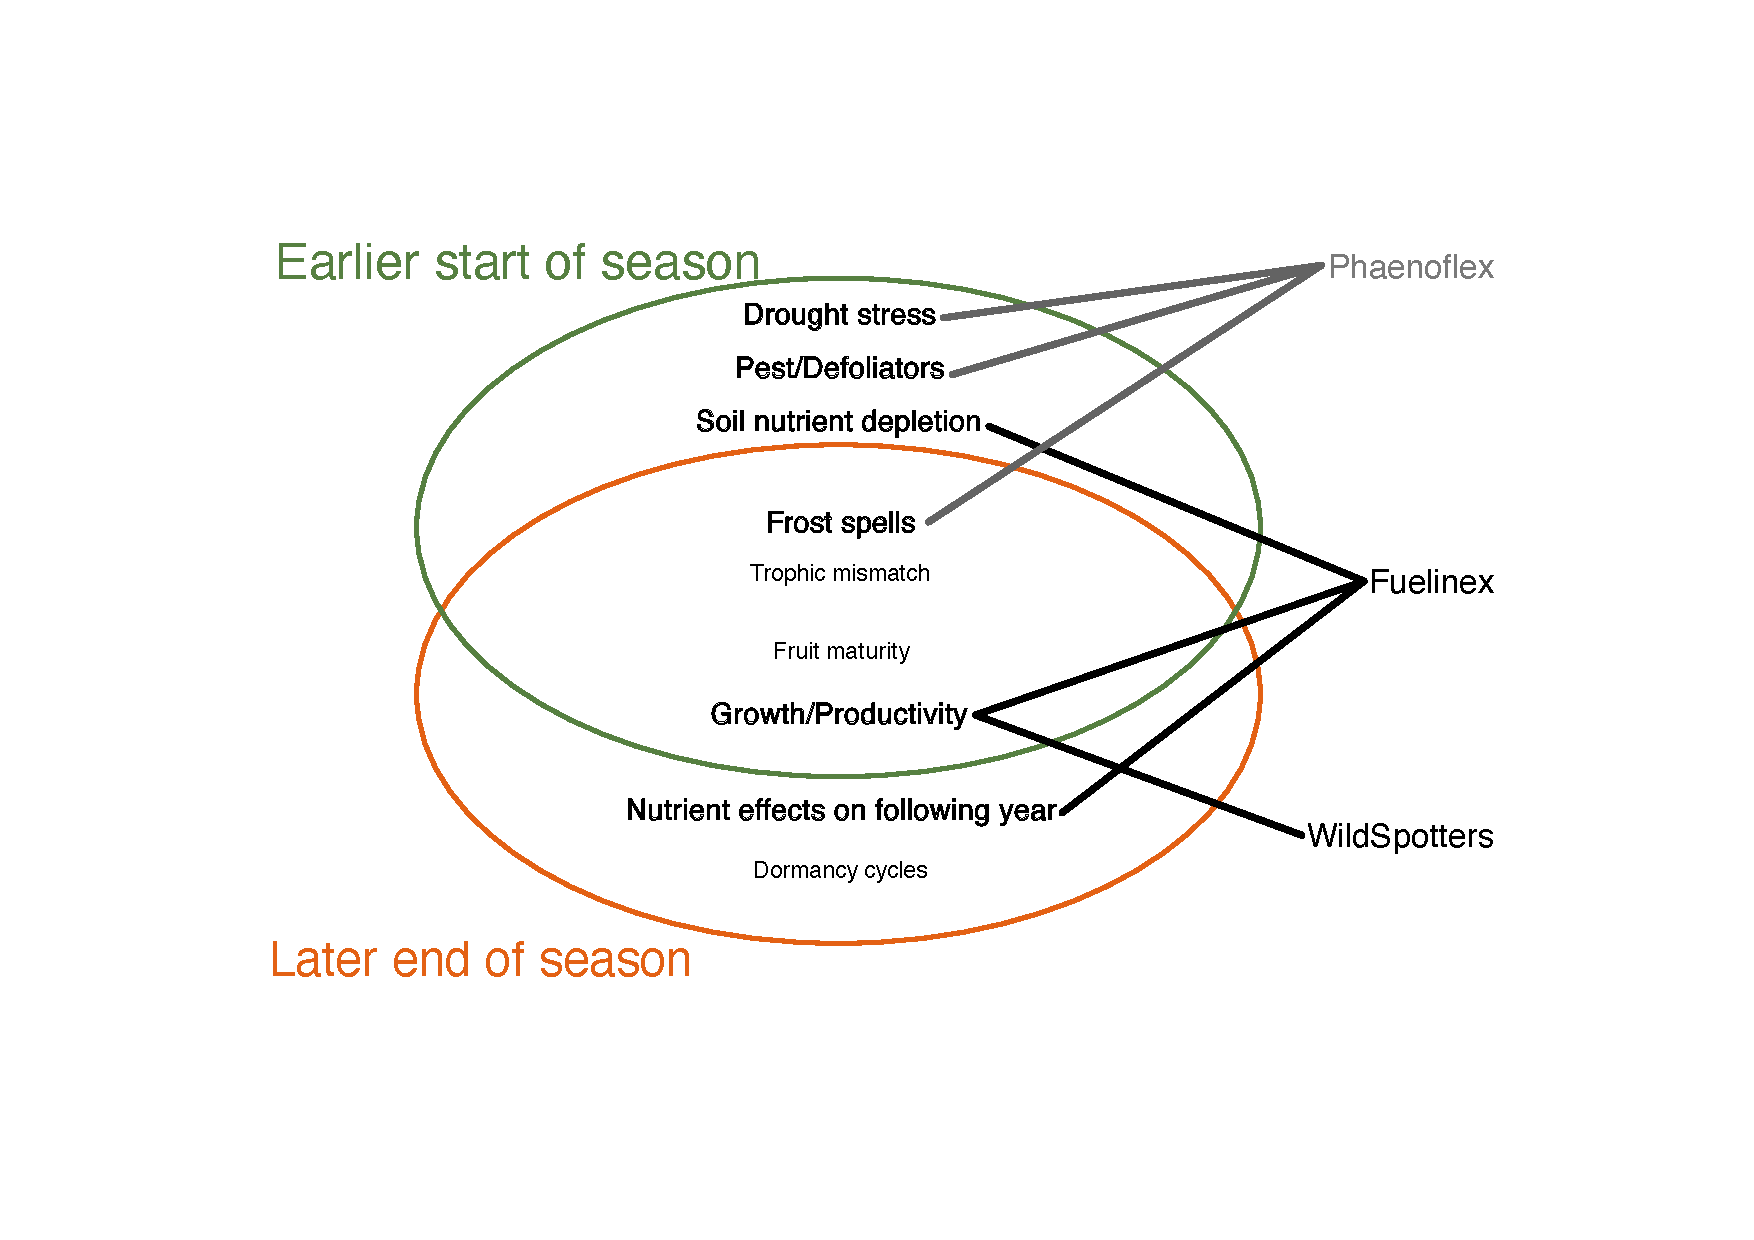
\includegraphics[width=1.1\textwidth]{studiedEffectsGSL.pdf}
\caption{The effects that an earlier start and later end of season can have on trees. In bold are the effects that were studied over the course of this thesis. Phaenoflex (in grey) is a related experimental project, that is not part of this thesis, but one I collaborated on in XX years.} %emwJan2 --explain your role in Phaenoflex a little? I added a clause you could fill in/expand on. 
\label{fig:sample}
\end{figure}

\clearpage
%<><><><><><><><><><><><><><><><><><><><><><><><><><><><><><><><><><><><><><><><>
% METHODOLOGY %
%<><><><><><><><><><><><><><><><><><><><><><><><><><><><><><><><><><><><><><><><>
\section{Methodology} %emwJan2 -- I did not get any of the below in my print out so did not review, but -- overall -- I think the above is close. If you can firm up the methods below and add some conceptual figures of the design or such then it should be good enough for your committee. If possible it would be nice to close on how these projects to the bigger open questions/problems you outline above (and in your conceptual figure (fig:sample)) but not critical. 

% <><><><><><><><><><><><><><><><><><><><><><><><><><><><><><>
% WILDCHROKIE %
% <><><><><><><><><><><><><><><><><><><><><><><><><><><><><><>
\subsection{Wildchrokie}
\textbf{2.1. Studies locations} \\
\textbf{Common garden}
*** what follows are the methods from the wildhell repo
In 2014-2015, we collected seeds from four field sites in northeastern North America spanning approximately a 3.5◦ latitudinal gradient. The four field sites included Harvard Forest (42.55◦N, 72.20◦W), the White Mountains (44.11◦N, 71.40◦W), Second College Grant, (44.79◦N, 71.15◦W), and St. Hippolyte, QC, CAN (45.98◦N, 74.01◦W). We transported all seeds back to the Weld Hill Research Building at the Arnold Arboretum in Boston Massachusetts (42.30◦N, 71.13◦W) where we germinated seeds following standard germination protocols, and grew them to seedling stages in the research greenhouse. In the spring of 2017 we out-planted seedlings to establish the garden. Plots were regularly weeded and watered throughout the duration of the study and were pruned in the fall of 2020.

In the spring of 2023, we collected cross-sections for most trees and 1 tree core on a few individuals. Both the cores and cross-sections were left to dry at ambient temperature for three months.

\textit{Phenological monitoring}
For the years of 2018-2019, we made phenological observations of all individuals in the common garden twice per week from February to December. In 2020 due to the COVID 19 pandemic, we monitored once per week from March to November. We describe phenological stages using a modified BBCH scale \citep{Finn2007} a common metrics for quantify woody plant phenological progression. We observed all major vegetative stages (budburst BBCH 07, leafout BBCH 15, end of leaf expansion BBCH 19, leaf coloration/drop BBCH 97, reproductive phases flowering BBCH 60-65, fruiting BBCH 72-79 and fruit/cones fully ripe BBCH 89). We added additional phases for budset and labelled full budset as BBCH 102.

% <><><><><><><><><><><><><><><><><><><><><><><><><><><><><><>
% CORINGTREESPOTTERS %
% <><><><><><><><><><><><><><><><><><><><><><><><><><><><><><>
\textbf{Coringtreespotters}
The Treespotters is a citizen science program that started in 2015 and aimed to train citizen scientist for accurate and rigorous phenological monitoring. From 2015 to 2024, hundreds of citizen scientists monitored 50 trees of 11 species regularly from budburst in the spring to leaf colouring in the fall. The BBCH scale was used (check if that's true). Not all phenophase was recorded for every tree, for every year, and some trees miss several several years of data. 

From 20 to 22 April 2025, we collected two 5-mm diameter core, 15-cm length at 1.3 meter above ground from 50 trees of the 11 species (Table XX) that were previously monitored for phenology, using an increment borer (Mora Borer, Haglöfs Sweden, Bromma, Stockholm, Sweden). The cores were collected perpenticularly to the slope and at 180 degrees from each other. We cleaned the increment borer with alcohol (70\% ethanol?) and the inside with a brush before collecting each core. We stored the cores in paper straws that were previously labelled and punched to help drying. They were stored at ambient temperature for three months. 

\textbf{Sample processing, imaging and measuring for WildSpotters}
We mounted the cores on wooden mounts, and sanded the cores and cross-sections using progressvely fine grit (150, 300, 400, 600, 800, 1000). We scanned the cores and cross-sections at a resolution of ***dpi using a homemade great scanner (Tina2026?)
We used the digitalized images to measure the tree ring widths with Fiji Image J. Then, we performed visual crossdating using Dplr, but no statistical crossdating was performed because of the short chronologies that limit the capacity for these analyses.

\textbf{Statistical analyses}
% <><><><><><><><><><><><><><><><><><><><><><><><><><><><><><>
% FUELINEX %
% <><><><><><><><><><><><><><><><><><><><><><><><><><><><><><>
\subsection {Fuelinex}
The experimental design of fuelinex is described in the figure.



%<><><><><><><><><><><><><><><><><><><><><><><><><><><><><><><><><><><><><><><><>
% SUPPLEMENTAL MATERIAL %
%<><><><><><><><><><><><><><><><><><><><><><><><><><><><><><><><><><><><><><><><>
\section {Supplemental material}

% --- --- --- --- --- --- --- --- --- --- --- --- --- --- --- ---
% SPECIES TABLES  %
% --- --- --- --- --- --- --- --- --- --- --- --- --- --- --- ---

%%%
\begin{table}[p]
\centering
\caption{Fuelinex species grouped by tree type, life history, and wood anatomy.}
\begin{tabular}{|>{\raggedright\arraybackslash}p{7cm}|p{5cm}|p{3cm}|p{1cm}|}
\hline
\multicolumn{4}{|c|}{\textbf{Deciduous Trees}} \\
\hline
\textbf{Common Name (Latin)} & \textbf{Life History Strategy} & \textbf{Wood Anatomy} & \textbf{n (approx)} \\
\hline
Bur oak (\textit{Quercus macrocarpa}) & Slow-growth, long life & Ring-porous & 87\\
Bitter cherry (\textit{Prunus virginiana}) & Fast-growth, short life & Diffuse-porous & 78\\
Box elder (\textit{Acer negundo}) & Fast-growth, short life  & Diffuse-porous & 90\\
Balsam poplar (\textit{Populus balsamifera}) & Fast-growth, short life  & Diffuse-porous &84 \\
Paper birch (\textit{Betula papyrifera}) & Fast-growth, short life  & Diffuse-porous &90\\
\hline
\multicolumn{4}{|c|}{\textbf{Evergreen Trees}} \\
\hline
White pine (\textit{Pinus strobus}) & Slow-growth, long life & & 89\\
Giant Sequoia (\textit{Sequoiadendron giganteum}) & Slow-growth, long life & & 54\\
\hline
\end{tabular}
\end{table}
%%%
% ============================
% Wildchrokie
% ============================
\subsection{Wildchrokie}
\begin {enumerate}
	\item Common garden from 2015 to 2023
	\item Four species within the Betulacea family (Table 2)
%%%
\begin{table}[p]
\centering
\caption{Wilchrokie species grouped by tree type, life history, and wood anatomy.}
\begin{tabular}{|>{\raggedright\arraybackslash}p{7cm}|p{5cm}|p{3cm}|p{1cm}|}
\hline
\multicolumn{4}{|c|}{\textbf{Deciduous Trees}} \\
\hline
\textbf{Common Name (Latin)} & \textbf{Life History Strategy} & \textbf{Wood Anatomy} & \textbf{n} \\
\hline
Paper birch (\textit{Betula papyrifera}) & Fast-growth, short life  & Diffuse-porous & 8\\
Yellow birch (\textit{Betula alleghaniensis}) & Moderate-growth, moderate life & Diffuse-porous & 21\\
Grey birch (\textit{Betula populifolia}) & Fast-growth, short life & Diffuse-porous & 29\\
Grey alder (\textit{Alnus incana}) & Fast-growth, short life & Diffuse-porous & 31\\
\hline
\end{tabular}
\end{table}
%%%
	\item Data: phenology, height, tree rings
	\item Analysis: Hierarchical model to understand how tree ring width relates to GDD
\end {enumerate}

% ============================
% Treespotters
% ============================
\subsection{Treespotters}
\begin {enumerate}
	\item Citizen scie nce project from 2015 to today (Table 3)
\begin{table}[h]
\centering
\caption{Treespotters species grouped by tree type, life history, and wood anatomy.}
\begin{tabular}{|>{\raggedright\arraybackslash}p{7cm}|p{5cm}|p{3cm}|p{1cm}|}
\hline
\multicolumn{4}{|c|}{\textbf{Deciduous Trees}} \\
\hline
\textbf{Common Name (Latin)} & \textbf{Life History Strategy} & \textbf{Wood Anatomy} & \textbf{n} \\
\hline
American basswood (\textit{Tilia americana}) & Fast-growth, moderate life & Diffuse-porous & 5\\
Eastern cottonwood (\textit{Populus deltoides}) & Fast-growth, short life & Diffuse-porous & 4\\
Northern red oak (\textit{Quercus rubra}) & Moderate-growth, long life & Ring-porous & 4\\
White oak (\textit{Quercus alba}) & Slow-growth, long life & Ring-porous & 5\\
Pignut hickory (\textit{Carya glabra}) & Slow-growth, long life & Ring-porous & 4\\
Shagbark hickory (\textit{Carya ovata}) & Slow-growth, long life & Ring-porous & 4\\
River birch (\textit{Betula nigra}) & Fast-growth, short life & Diffuse-porous & 5\\
Yellow birch (\textit{Betula alleghaniensis}) & Moderate-growth, moderate life & Diffuse-porous & 4\\
Sugar maple (\textit{Acer saccharum}) & Slow-growth, long life & Diffuse-porous & 5\\
Red maple (\textit{Acer rubrum}) & Slow-growth, long life & Diffuse-porous & 4\\
Yellow buckeye (\textit{Aesculus flava}) & Moderate-growth, moderate life & Diffuse-porous & 5\\
\hline
\end{tabular}
\end{table}
	\item Tree coring
	\item Data: phenology, tree rings
	\item Analysis: Hierarchical model to understand how tree ring width relates to GDD	
\end {enumerate}

% --- --- --- --- --- --- --- --- --- --- --- --- --- --- --- ---
% Tables spring frost, drought and heat waves $
% --- --- --- --- --- --- --- --- --- --- --- --- --- --- --- ---
\textbf{3.1. Spring frosts} \\
\resizebox{\textwidth}{!}{
\begin{tabular}{|>{\raggedright\arraybackslash}p{4cm}|p{12cm}|}
\hline
\textbf{Definition:} &  Late spring frosts are below-freezing temperatures in late spring \citep{zohner_late-spring_2020} \\
\hline
\textbf{Mechanisms} & Early warm spells $\rightarrow$ early leaf out $\rightarrow$ hard frost ($<$-2Celsius) $\rightarrow$ tissue death = loss of photosynthetic capacity \citep{polgar_leafout_2011}; Response: second cohort of leaves are more efficient and mitigate carbon sequestration loss \citep{reinmann_compensatory_2023} \\
\hline
\textbf{Global trend of occurrence} & Most vulnerable regions are the ones with no past risk of occurrence (); $\uparrow$ in Europe and East Asia, but $\downarrow$ North America; Global trend is controversial \citep{reinmann_compensatory_2023} \\
\hline
\textbf{Consequences (Individual and Ecosystem level consequences)} & Loss of vegetative tissue = $\downarrow$ photosynthesis = $\downarrow$ and remobilization of NSC to repair damaged tissues = $\downarrow$ secondary growth \citep{meyer_frost_2024}; Loss of reproductive tissue (higher flower mortality) \citep{sgubin_risk_2018}; Costs for orchards and stuff \citep{reinmann_compensatory_2023} \\
\hline
\textbf{Differences across species/provenance} & \\
\hline
\end{tabular}
} 

\clearpage
	\textbf{3.2. Drought} \\
\resizebox{\textwidth}{!}{
\begin{tabular}{|>{\raggedright\arraybackslash}p{4cm}|p{12cm}|}
\hline
\textbf{Definition:} &  "Drought is a prolonged absence or marked deficiency of precipitation that results in water shortage or or a period of abnormally dry weather sufficiently prolonged for the lack of precipitation to cause a serious hydrological imbalance \citep{trenberth_global_2014,intergouvernemental_panel_on_climate_change_climate_2007}. \\
\hline
\textbf{Mechanisms} & — Hot temperature + low precipitation (aka global-change-type drought \citep{tyree_xylem_2002})= $\uparrow$ evapotranspiration$\rightarrow$ less water in soil $\rightarrow$ cavitation $\rightarrow$ embolism $\rightarrow$ hydraulic failure \citep{tyree_xylem_2002} = tissue death \citep{choat_triggers_2018}; 

— Earlier spring phenology = longer GS $\rightarrow$ increases vegetative growth $\rightarrow$ increases evapotranspiration $\rightarrow$ increases drawdown of soil moisture = progressive water stress \citep{li_widespread_2023}

— Long-term vs short-term stomatal responses and consequences on tissue death \citep{choat_triggers_2018}; 

— Recovery and its determinants \citep{choat_triggers_2018,li_widespread_2023}\\
\hline
\textbf{Global trend of occurrence} & — $\uparrow$ precipitation anomalies since 1990 \citep{trenberth_global_2014};  

— Models often exclude PDO/ENSO which limit the capacity to attribute increasing droughts to CC  \citep{trenberth_global_2014}; 

— Weak evidence of detection and attribution of changes in meteorological drought since the mid-20th century \citep{intergovernmental_panel_on_climate_change_detection_2014}; 

— Using a spacial, model-based perspective, anthropogenic forcing increased the frequency, duration and intensity of SPI-based droughts for North America \citep{hidalgo_detection_2009}, Europe and the Mediterreanean \citep{spinoni_will_2018}, \citep{kurnik_testing_2011} and E Asia  \citep{chiang_evidence_2021,marvel_twentieth-century_2019,spinoni_world_2014}\\
\hline
\textbf{Consequences (Individual and Ecosystem level consequences)} & — Recurring droughts may limit trees' ability to recover from other types of stress.

—Tree mortality (e.g. Texas and California extreme droughts are estimated to have killed 300 and 102 million trees \citep{li_widespread_2023})\\ 
\hline
\textbf{Differences across species/provenance} &  \\
\hline
\end{tabular}
} \\
\par

\textbf{3.3. Heat waves}\\
\resizebox{\textwidth}{!}{
\begin{tabular}{|>{\raggedright\arraybackslash}p{4cm}|p{12cm}|}
\hline
\textbf{Definition:} &  Heat wave is a period of excessively hot weather (5 or more consecutive days of prolonged heat in which the daily maximum temperature is higher than the average maximum temperature by 5 °C ), which may be accompanied by high humidity \citep{marx_heat_2021}. \\
\hline
\textbf{Mechanisms} &  $\uparrow$ atmospheric CO2 = $\uparrow$ temperature $\rightarrow$ $\uparrow$ heat waves... More specifically: A mechanism for the increase occurence of heat waves is a weakeking of the polar jet stream (important weather factor for middle latitude regions of North America, Europe and Asia) caused by global warming which increases the occurence of stationnary weather, resulting in heavy rain falls or heat waves \citep{marx_heat_2021}.  Extreme heat $\rightarrow$ growth either through (1) Directly via cell processes disruption or (2) indirectly via effects of rising leaf-to-air vaport deficit (VPD) \citep{gagne_limited_2020}.

Increased temperature leads to reduced photosynthesis which can be attributed to: 
1. Damage to photosynthetic machinery
2. Inactivation of RUBISCO
3. R eduction to RuBP regeneration
4. Membrane stability 
5. Increased mitochondrial respiration and photorespiration \citep{hauck_heat_2025}
\\
\hline
\textbf{Global trend of occurrence} & Heat waves have increased \citep{gagne_limited_2020,meehl_more_2004,teskey_responses_2015} and are expected to increase under future climate change \citep{dosio_extreme_2018,intergovernmental_panel_on_climate_change_detection_2014,teskey_responses_2015}. Summertime extreme temperatures associated with prolonged heat waves, lasting for several weeks, now impact approximately 10\% of land surfaces, up from only 1\% in the 1960s. \citep{teskey_responses_2015}.
The more intense and more frequently occurring heat waves cannot be explained solely by natural climate variations and without human-made climate change \citep{marx_heat_2021}.
 \\

\hline
\textbf{Consequences (Individual and Ecosystem level consequences)} &  - Reduced photosynthesis  - Increased mortality - Photosynthetic tissue loss \citep{gagne_limited_2020}.\\ 
\hline
\textbf{Differences across species/provenance} & Some species have thermal photosynthetic/respiratory acclimatation while others don't. Growth and survival will change depending on species to thermally acclimate to both photosynthesis and respiration 
- This is explained by growth strategies of gymnosperms vs angiosperms (which are usually better)
 \\
\hline
\end{tabular}
}



% --- --- --- --- --- --- --- --- --- --- --- --- --- --- --- ---
% References %
% --- --- --- --- --- --- --- --- --- --- --- --- --- --- --- ---

\bibliography{ExportedItems}
\bibliographystyle{ecolett} 

\end{document}
